\documentclass[11pt,a4paper,headsepline,footsepline,bibliography=totocnumbered]{article}

\usepackage[utf8]{inputenc}
\usepackage{lmodern}
\usepackage[ngerman]{babel}
\usepackage[T1]{fontenc}
\usepackage[left=2.5cm,right=2.5cm,top=2.5cm,bottom=2.5cm]{geometry}
\usepackage{microtype}
\usepackage{bookmark}

\usepackage{fancyhdr}
\usepackage[onehalfspacing]{setspace}
\usepackage[font=small]{caption}


% Abb. statt Abbildung als Caption
\addto\captionsngerman{\renewcommand{\figurename}{Abb.}}
% Tab. statt Tabelle als Überschrift
\addto\captionsngerman{\renewcommand{\tablename}{Tab.}}

\setlength{\headheight}{14pt}

\usepackage{chngcntr}
\counterwithout{equation}{section}
\renewcommand{\theequation}{\arabic{equation}}

%change font
\renewcommand{\familydefault}{\sfdefault}

\usepackage{tikz} %Zum Diagramme zeichnen
\usepackage{pgfplots}
\pgfplotsset{compat=1.17}

\setlength{\parindent}{0cm} % Einrückung bei Paragraphenbeginn entfernen

%%%

\begin{document}
\pagestyle{fancy}
\pagenumbering{arabic}

\thispagestyle{empty}

\begin{center}
  \begin{figure}[h]
    
\includegraphics[width=5cm]{pictures/htw-logo.png}
  \end{figure}

  \vspace{0.25cm}

  \huge{HTW Berlin}
  \linebreak
  \Large{Fachbereich 4 - Informatik, Kommunikation und Wirtschaft}
  \linebreak
  \Large{BA - Angewandte Informatik}
  \linebreak

  \vspace{0.25cm}

  \textbf{\Huge{Semesterbegleitende Arbeit - KilterVote}}

  \vspace{0.25cm}

  \Large{B35 - Mobile Betriebssysteme und Netzwerke}
  \linebreak
  \large{WiSe - 24/25}
  \linebreak
  \large{Prof. Dr. Thomas Schwotzer}
\end{center}

\vspace{1cm}

% \begin{verbatim}
% \end{verbatim}

% \begin{verbatim}
% \end{verbatim}

\begin{flushleft}
\begin{tabular}{lll}
  \textbf{Bearbeitende:} & & Yannik Schüler \\ & & Simon Cornelius \\
  \textbf{Matrikelnummern:} & & 583880 \\ & &  577602 \\
\end{tabular}


\end{flushleft}

\pagebreak
\tableofcontents

\newpage

\section{Projektidee}

  \subsection{Beschreibung}
    \par
      Die Applikation soll zum Wählen von Routen am Kilter Board in einer Boulderhalle helfen,
      denn oftmals ist es schwer eine unparteiische Wahl zwischen verschiedenen Schwierigkeitsgeraden der Routen zu gewährleisten -
      gerade wenn eine weite Spanne von Erfahrungsstufen unter den Boulderern vertreten ist.
      Jeder Boulderer kann Routen zu einem Auswahl-Pool hinzufügen und diese mit einem bestimmten Schwierigkeitsgerad versehen,
      dann kann jeder Boulderer für eine Route stimmen und ein Wahl-Algorithmus, basierend auf den Erfahrungsstufen der Teilnehmer, wählt dann eine Route aus.
      Während des Kletterns tragen die Boulderer ihre Versuche auf jeder Route in die App ein, um am Ende eine Auswertung zu erhalten.
      Auf Wunsch können die persönlichen Statistiken auch gespeichert werden, sowie Statistiken zwischen bestimmten Boulderern (Rivalitäten).

    \subsubsection{Use Cases}
      \begin{enumerate}
        \item Session erstellen oder einem Session beitreten durch Angabe eines Session Codes (möglicherweise auch via NFC)
        \item Angabe eines Namens und dem eigenen Erfahrungslevel im Bouldern
        \item Hinzufügen k/einer oder mehrerer Routen zum Route Pool
        \item Ansehen der verschiedenen Routen im Pool
        \item Wählen für eine Route
        \item Loggen der Versuche mit Fortschritt (in Prozenten), sowie dem Erreichen eines Checkpoints
        \item Ändern des eigenen Erfahrungslevels während einer laufenden Session
        \item Anzeigen von Statistiken der aktuellen Session
        \item Verlassen der laufenden Session
      \end{enumerate}

    \subsubsection{Use Case Diagram}
      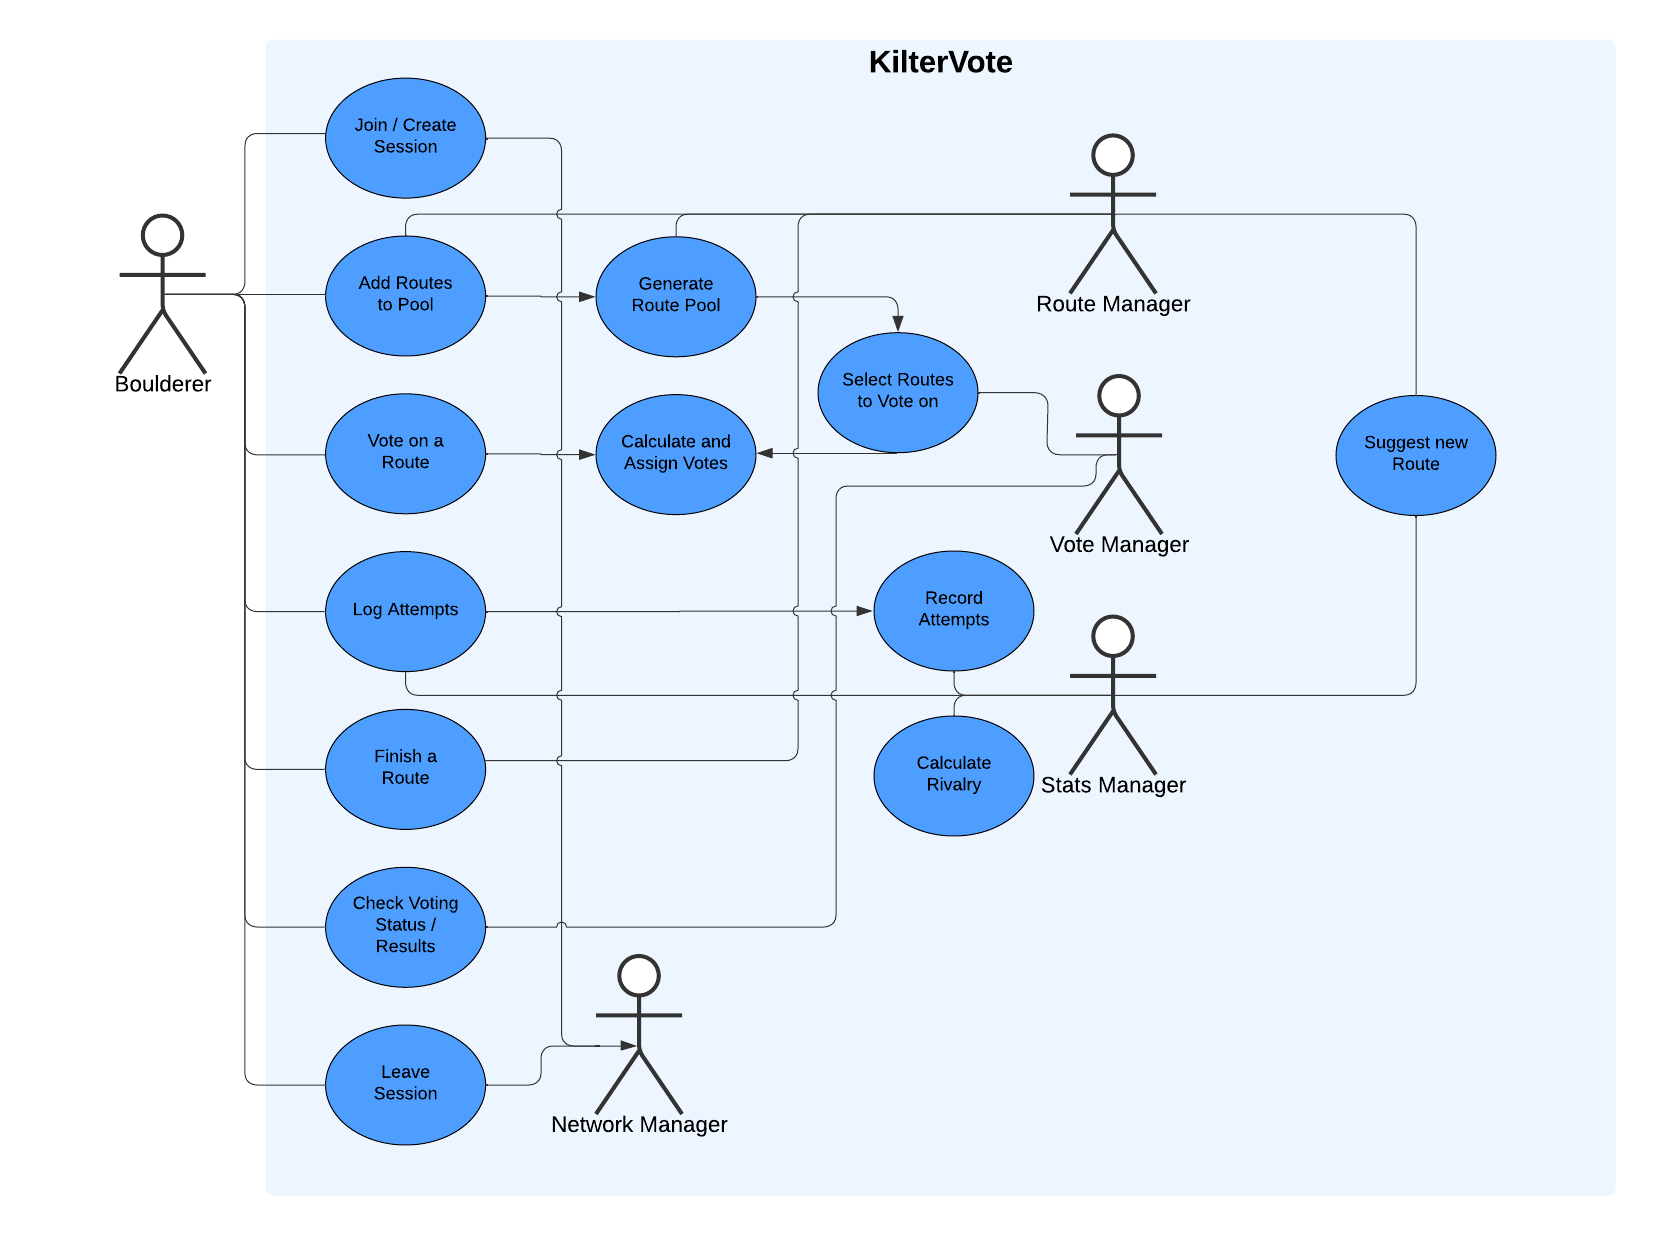
\includegraphics[width=\textwidth]{pictures/Use_Case_Diagram.png}

  \subsection{Einordnung in die Anforderungen}  
    \par  
      Die Applikation basiert auf einem Ad-hoc Netzwerk welches zwischen den Geräten der Boulderer aufgebaut wird.
      Dafür ziehen wir Bluetooth, sowie WiFi-Direct in Betracht, im Optimalfall wird die Möglichkeit für beides geboten.
      Die Statistiken der Boulderer und die Versuche während der Sessions werden auf dem persönlichen Gerät gespeichert und dann im Ad-hoc Netzwerk gepublished, somit liegen die Daten immer verteilt auf mehreren Geräten.
      Lässt es der zeitliche Rahmen zu besteht auch die Möglichkeit NFC für das Beitreten/Erstellen einer Session zwischen Boulderern zu nutzen.
    
  \subsection{Wireframes}
    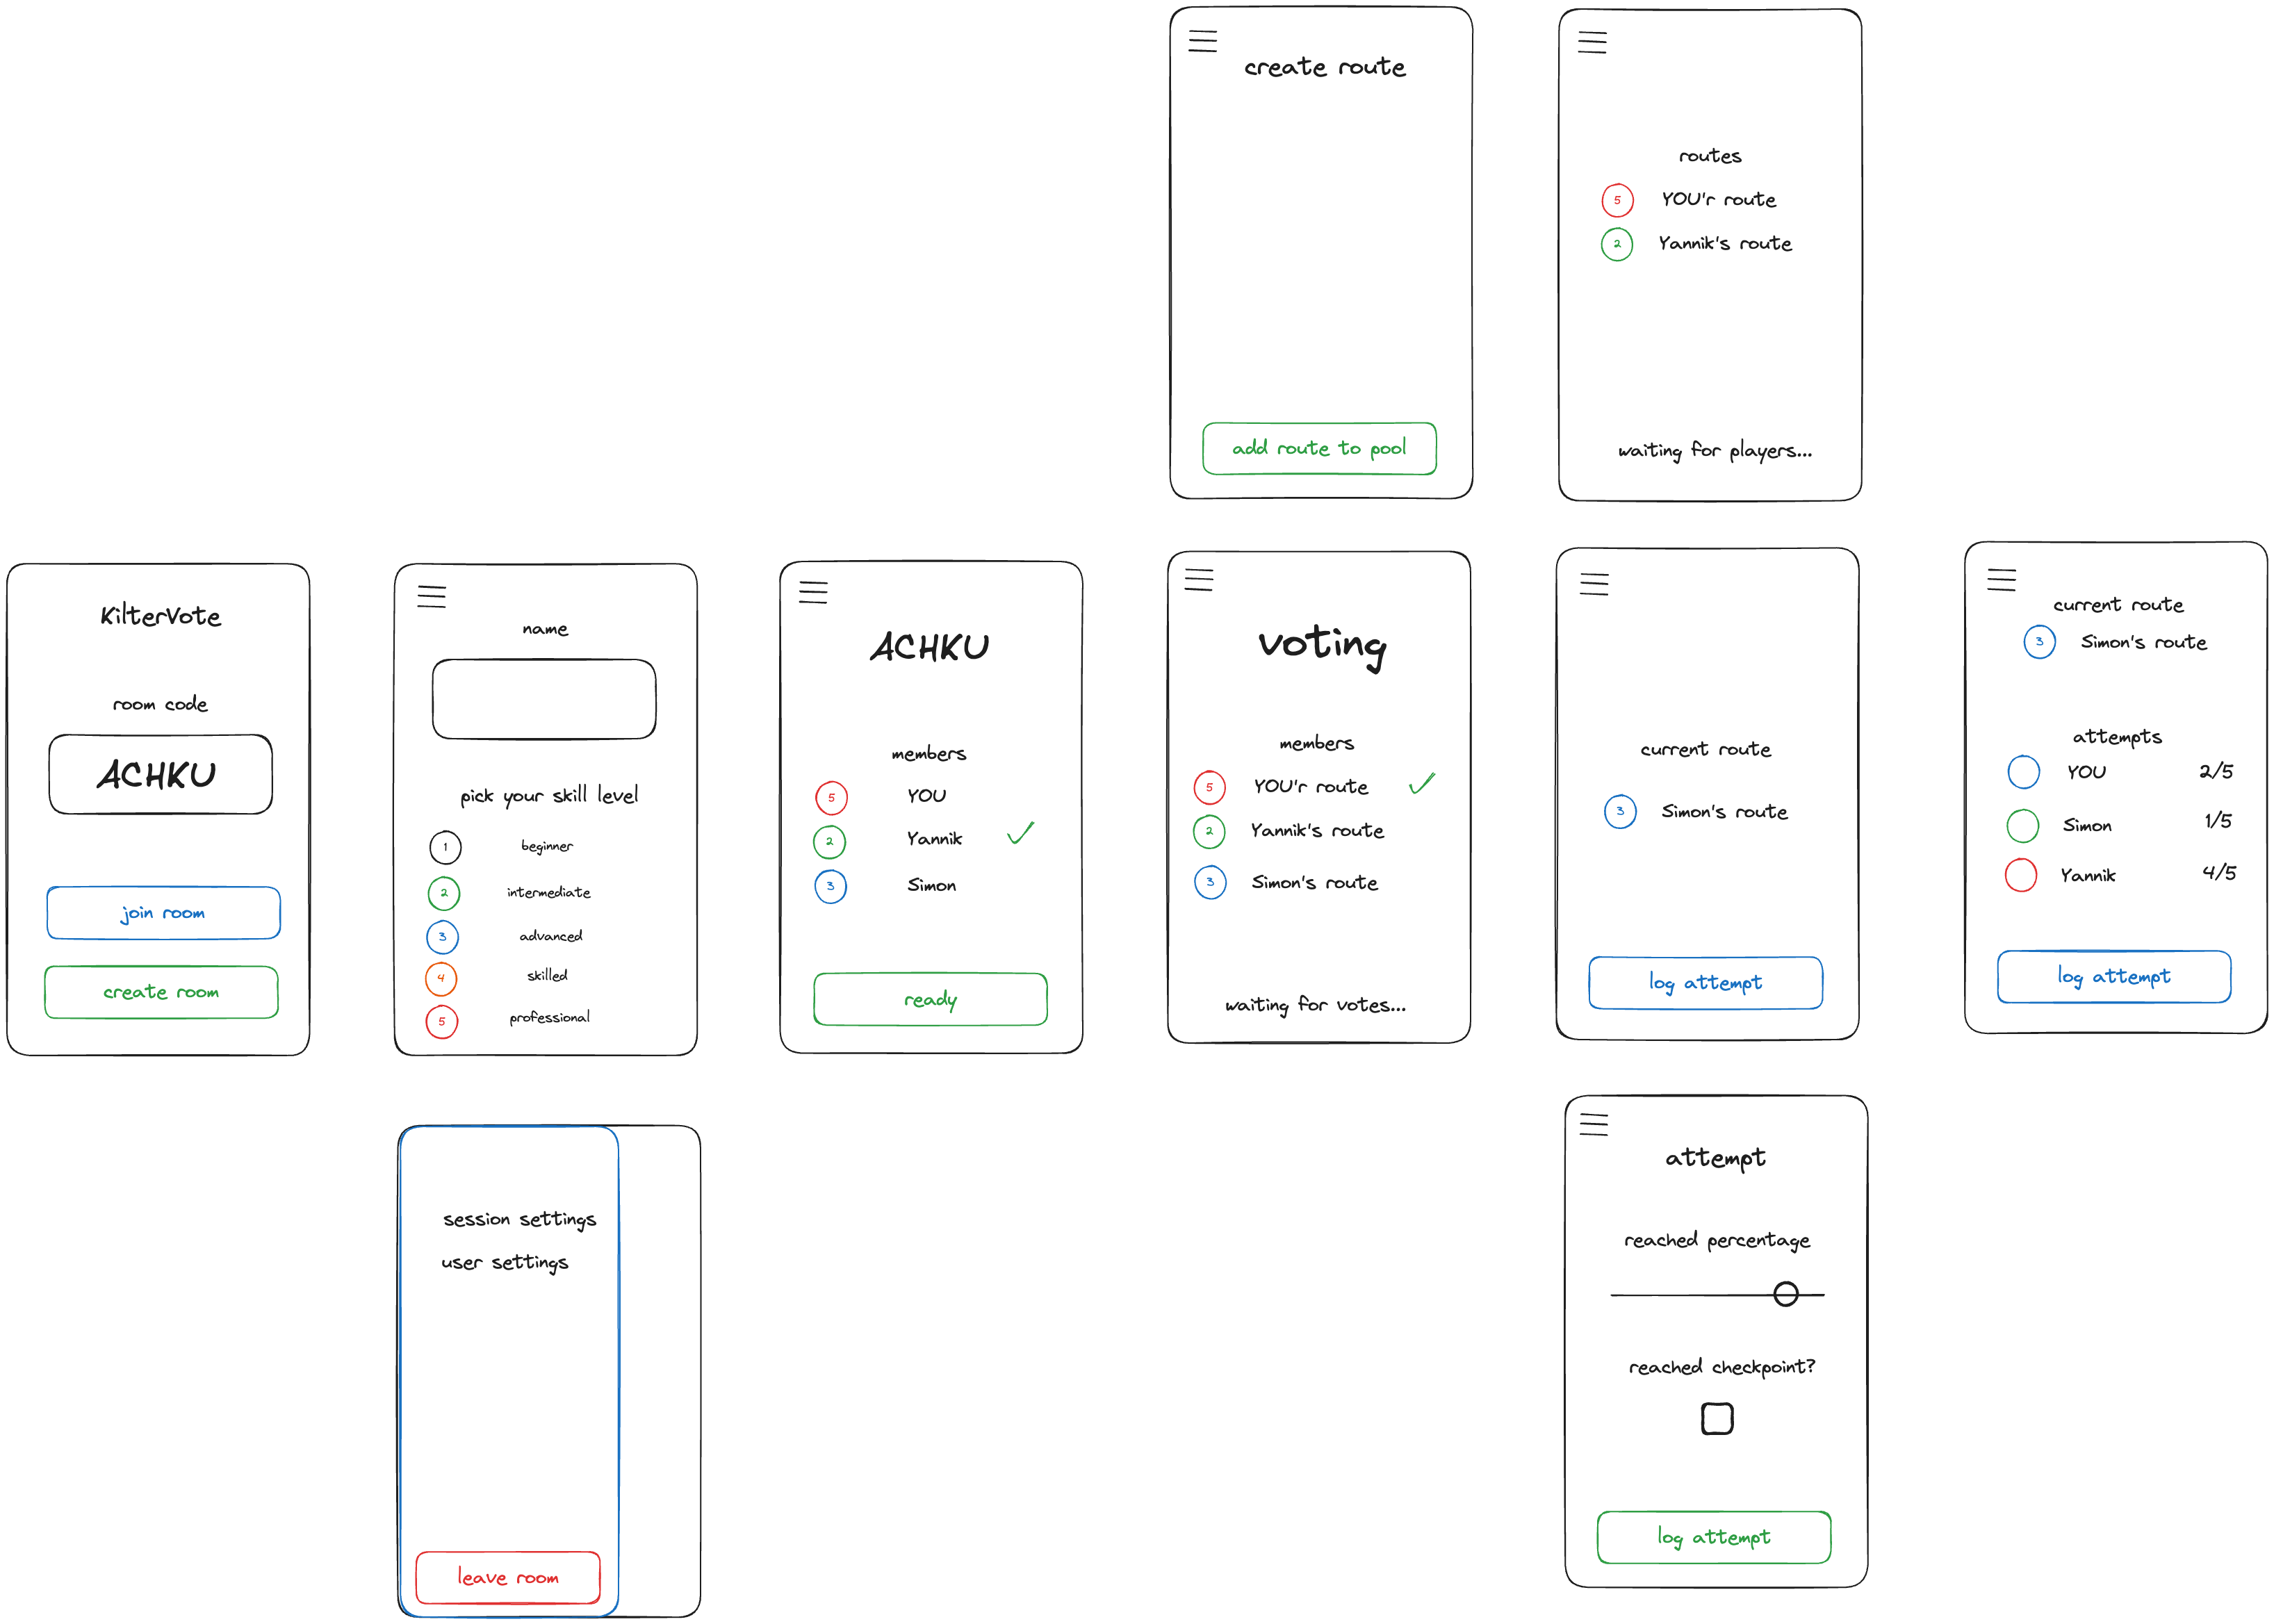
\includegraphics[width=\textwidth]{pictures/KilterVote_GUI.png}

\end{document}
